\section{Control as Inference}
This is a brief exploration into the question of what constitutes optimal behaviour. Traditionally, we’ve 
assumed that the behaviour we want to imitate is perfectly optimal. However, this assumption is not realistic
since humans rarely act in strictly optimal ways.\newline
In this section, we explore Control as Inference, a paradigm that reimagines reinforcement learning not as a strict 
reward-maximisation problem, but as an inference problem within a probabilistic framework. This approach allows us to 
model and tolerate sub-optimal behaviour. We begin with an introduction to variational inference which forms the 
foundation for this reformulation

\subsection{Variational Inference}
A central challenge in modern statistics, especially Bayesian statistics, is approximating complex, intractable 
probability distributions, such as posterior densities like 
$$p(z|x) = \frac{p(x|z)p(z)}{p(x)} = \frac{p(x|z)p(z)}{\int_z p(x,z')\, dz'}$$
where $z$ represents the latent variables and $x$ represents the observed data. The marginalization over $z$ to 
calculate $p(x)$ in the denominator is typically intractable, because, for example, the search space of $z$ is too 
large. Traditional methods like Markov Chain Monte Carlo offer accurate sampling but are often computationally 
expensive, particularly for large datasets or complex models. \newline
Variational Inference (VI) provides a faster alternative by reframing inference as an optimization problem. Instead 
of sampling, VI approximates the true posterior by selecting the closest distribution $q_\theta(z)$ (from a simpler, 
predefined family) using a dissimilarity measure such as Kullback-Leibler (KL) divergence in order to find 
the best paramerters $\theta$.\newline 
In the following, we will explore how the most common discrepancy measure, the Kullback-Leibler divergence, can be 
used for inference. Additionally, in the upcoming discussion, $p^*(x)$ will represent the true probability 
distribution, while  $q(x)$ will denote the approximation.

\subsubsection{Minimizing Reverse KL}
Minimizing the reverse KL divergence is often referred to as (I)nformation-projection and is defined as:
$$\text{KL}(q(x)||p^*(x)) = \int_x q(x)\log{\frac{q(x)}{p^*(x)}} \diff x$$
This objective is also known for its zero-forcing behaviour. This term arises from how the reverse KL divergence 
behaves in regions where the true distribution $p^*(x)$ has high probability mass, but the approximate distribution 
$q(x)$ assigns little or no mass. Consider two cases:
\begin{itemize}
    \item If $p^*(x) > 0$ but $q(x) \approx 0$, then the ratio $\frac{q(x)}{p^*(x)}$ inside the logarithm becomes 
    very small. However, since $q(x) \log(\cdot)$ is multiplied by a value close to zero, the overall contribution to 
    the KL divergence is negligible.    
    \item If $q(x) > 0$ and $p^*(x) = 0$, then the ratio becomes infinite, and $\log(\infty) = \infty$. This causes 
    the 
    KL divergence to become infinitely large, leading the optimization to avoid placing mass in such regions.
\end{itemize}
Therefore, minimizing the reverse KL forces $q(x)$ to avoid assigning probability mass where $p^*(x) = 0$. This 
behavior leads to mode-seeking: reverse KL tends to concentrate $q(x)$ on one mode of $p^*(x)$, ignoring regions of 
low probability. And as long as we are able to sample from $q(x)$, we can approximate the KL divergence using Monte 
Carlo integration.

\subsubsection{Minimizing Forward KL}
Minimizing the forward KL divergence is often referred to as (M)oment-projection and is defined as:
$$\text{KL}(p^*(x)||q(x)) = \int_x p^*(x)\log{\frac{p^*(x)}{q(x)}} \diff x$$
This objective exhibits probability forcing: if the true distribution $p^*(x)$ is high in a region, 
then the approximation $q(x)$ must also be high there to avoid a large penalty. So it got the following properties:
\begin{itemize}
    \item It tends to average over multiple modes of $p^*(x)$, even when the approximation family cannot represent 
    such multimodality well.
    \item It requires samples from the true distribution $p^*(x)$, making it generally unsuitable for variational 
    inference 
    $$ \int_x p^*(x)\log{\frac{p^*(x)}{q(x)}} \diff x = \mathbb{E}_{\color{red}x \sim p^*(x)}\left[\frac{p^*(x)}{q(x)}\right]$$
    \item Minimizing the forward KL is equivalent to maximum likelihood estimation (MLE).
    $$ \int_x p^*(x)\log{\frac{p^*(x)}{q(x)}} \diff x = \text{const }- \int_x p^*(x)\log{q(x)} \diff x$$
\end{itemize}

\begin{figure}[H]
    \centering
    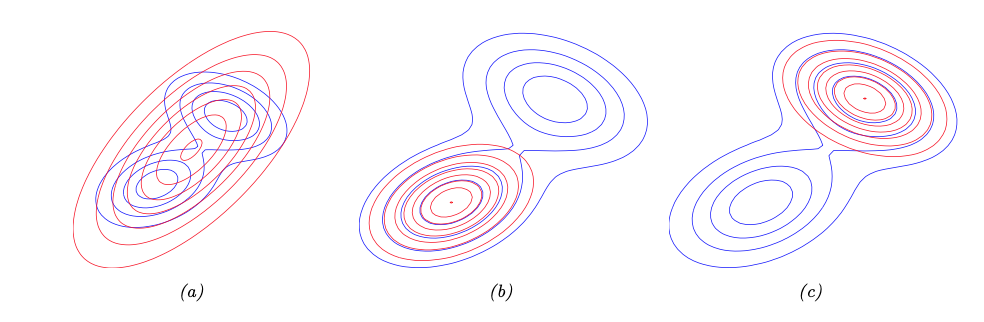
\includegraphics[width=0.9\linewidth]{images/rev_forw_kl.png}
    \caption{Illustrating forward vs. reverse KL. The blue contours represent the true distribution $p^*$, 
    and the red contours are from the approximation $q$. (a) Minimizing forward KL. (b–c) Minimizing reverse KL, 
    where $q$ fits onto different modes each time. }
    \label{fig:reverse_vs_forward_kl}
\end{figure}

\subsection{Connection between Variational Inference and Control}
As mentioned earlier, our current understanding does not allow us to account for suboptimal behaviour in our algorithms. Consider, for 
example, a task where we are required to move a dot on a screen to a goal using a joystick. The optimal behaviour in this scenario would
be to take the straight path, but small deviations may occur due to factors such as lack of concentration or external distractions. Despite
these deviations, we still achieve the same outcome as if we had followed the optimal path. Intuitively, we recognize that small errors do 
not necessarily prevent the task from being successfully completed. Therefore, it is clear that some mistakes are more consequential than 
others when completing a task while still achieving the overall goal.\newline
To incorporate suboptimality into our model, we begin by adding the concept of optimality to the general structure of a MDP. We introduce an 
optimality variable $o_t$, where $o_t = 1$ indicates that time step $t$ is optimal, and $o_t = 0$ indicates that it is not. The corresponding 
graphical model is illustrated as follows
\begin{figure}[H]
    \centering
\resizebox{!}{3.25cm}{
\begin{tikzpicture}
\tikzset{
  main/.style={circle, minimum size = 5mm, thick, draw =black!80, node distance = 20mm},
  connect/.style={-latex, thick},
  box/.style={rectangle, draw=black!100}
}
  \node[main] (L1) [] {$S_1$};
  \node[main] (L2) [right=of L1] {$S_2$};
  \node[main] (L3) [right=of L2] {$S_3$};
 % \node[main] (Lt) [right=40mmof L3] {$S_t$};
  \node[] (Lhid) [right=17mmof L3] {$\dots$};
  
\node[main] (A1) [below right=10mm of L1] {$A_1$};
\node[main] (A2) [below right=10mm of L2] {$A_2$};
\node[main] (A3) [below right=10mm of L3] {$A_3$};
%\node[main] (At) [below left=10mm of Lt] {$A_{t-1}$};


  \node[main,fill=black!10] (O1) [below=of L1] {$O_1$};
  \node[main,fill=black!10] (O2) [below=of L2] {$O_2$};
  \node[main,fill=black!10] (O3) [below=of L3] {$O_3$};
  %\node[main,fill=black!10] (Ot) [below=of Lt] {$O_t$};
  \path (L1) edge [connect] (L2)
        (L2) edge [connect] (L3)
        (L3) edge [connect] (Lhid);
        %(Lhid) edge [connect] (Lt);
        
  \path (A1) edge [connect] (O1)
        (A1) edge [connect] (L2)
        (A2) edge [connect] (O2)
        (A2) edge [connect] (L3)
        (A3) edge [connect] (O3)
        (A3) edge [connect] (O3)
        (A3) edge [connect] (Lhid);
        %(At) edge [connect] (Lt);
  \path (L1) edge [connect] (O1);
  \path (L2) edge [connect] (O2);
  \path (L3) edge [connect] (O3);
  %\path (Lt) edge [connect] (Ot);
\end{tikzpicture}}

\end{figure}
This model resembles a Hidden Markov Model. We now define some probabilities, which may initially appear arbitrary. 
However, they will lead to an elegant framework. For now, we take them as given:
\begin{gather*}
    p(\tau) = p(s_1, a_1, \dots, s_T) = p(s_1) \prod_{t=1}^{T-1} p(s_{t+1} \mid s_t, a_t) \underbrace{\pi(a_t \mid s_t)}_{1\ 
    \text{(uniform)}} \\
    p(o_t \mid s_t, a_t) \propto \exp(r(s_t, a_t)) \\
    p(o_{1:T} \mid \tau) = \exp\left(\sum_{t=1}^T r(s_t, a_t)\right)
\end{gather*}
Our goal is to infer the most likely trajectory given that the agent acts optimally. This means we want to compute 
the posterior:
\begin{equation}
    p(\tau \mid o_{1:T} = 1) = \frac{p(\tau)\,p(o_{1:T} = 1 \mid \tau)}{p(o_{1:T} = 1)} \label{infer_poste}
\end{equation}
Once we have this posterior, we can use marginalization and conditioning to compute the optimal policy:
$$p(a_t \mid s_t, o_{1:T} = 1)$$
The distribution \eqref{infer_poste} can be challenging to compute directly, so we turn to variational inference. 
Specifically, we minimize the reverse KL divergence between an approximate distribution $q_\theta(\tau)$ and the true 
posterior.\newline
We define our variational distribution $q_\theta(\tau)$ as follows (again, this form might seem arbitrary, but it is 
motivated by deeper theory—see resources for details):
$$
q_\theta(\tau) = p(s_1) \prod_t p(s_{t+1} \mid s_t, a_t)\, q_\theta(a_t \mid s_t)
$$
Minimizing the reverse KL divergence gives us the following objective:
\begin{align*}
    \text{KL}(q_\theta(\tau)|| p(\tau|o_\tau=1)) &= \int q_\theta(\tau) \log{ \frac{p(\tau){p(o_\tau=1 | \tau)}}{q_\theta(\tau)\color{green!50!black}p(o_\tau=1)}} \diff \tau \\
    &=\int q_\theta(\tau)\log{p(o_\tau|\tau)}\diff \tau - \text{KL}(q_\theta(\tau)||p(\tau)) + \text{\color{green!50!black}const} \\
    &=\int q_\theta(\tau)\log{p(o_\tau|\tau)}\diff \tau - \int q_\theta(\tau)\log{\frac{q_\theta(\tau)}{p(\tau)}}\diff \tau \\
    &= \int  q_\theta(\tau) \left(\log{p(o_\tau|\tau)} - \log{\frac{q_\theta(\tau)}{p(\tau)}}\right) \diff \tau \\
    &= \int  q_\theta(\tau) \left(\log{p(o_\tau|\tau)} - \log{\frac{ p(s_1)\prod_t p(s_{t+1}|s_t,a_t)q_\theta(a_t|s_t)}{ p(s_1) \prod_{t}p(s_{t+1}|s_t,a_t)}}\right) \diff \tau \\
    &=\int  q_\theta(\tau) \left(\log{p(o_\tau|\tau)} - \log{\prod_t q_\theta(a_t|s_t)}\right) \diff \tau \\
    &=\int  q_\theta(\tau) \left(\log{\left(\exp(\sum_{t=0}^T r(s_t,a_t))\right)} - \log{\prod_t q_\theta(a_t|s_t)}\right) \diff \tau \\
    &=\int  q_\theta(\tau) \left(\sum_t r(s_t,a_t) -\log{q_\theta(a_t|s_t)}\right) \diff \tau \\
    &=  \mathbb{E}_{(s_{1:T},a_{1:T})\sim q_\theta}\left[\sum_t r(s_t,a_t) -\log{q_\theta(a_t|s_t)}\right] \\
    &=  \sum_t\mathbb{E}_{(s_t,a_t)\sim q_\theta}\left[r(s_t,a_t) +H(q_\theta(a_t|s_t))\right] 
\end{align*}
This objective is identical to the one encountered in maximum entropy reinforcement learning, specifically when we 
discussed Soft Actor-Critic (SAC) in Section~\ref{SAC}. In that sense, SAC can be interpreted as performing the 
expected information projection (I-projection).\newline
It’s worth noting that, in this setting, exact inference over the Hidden Markov Model (HMM) could also be performed 
using the forward-backward algorithm. However, we will not cover that here. For those interested, the resources 
provided include further materials that explore this topic in more depth.

\subsection{Resources}
A great introduction to variational inference can be found in \cite{Blei_2017}. Another excellent resource is 
''CS 285: Lecture 18 – Variational Inference`` by Sergey Levine, which provides an intuitive and accessible overview. 
In ''Lecture 19 – Control as Inference``, he derives many of the equations referenced above, which we treated as 
given, and shows how to perform \textbf{exact} inference using the forward-backward algorithm to compute the 
posterior \cite{CS285,CS285LevineYoutube}. Much of the material in these lectures is based on his tutorial 
Reinforcement Learning and Control as Probabilistic Inference 
\cite{levine2018reinforcementlearningcontrolprobabilistic}.